\documentclass[border=10pt]{standalone}
\usepackage{tikz}
\begin{document}
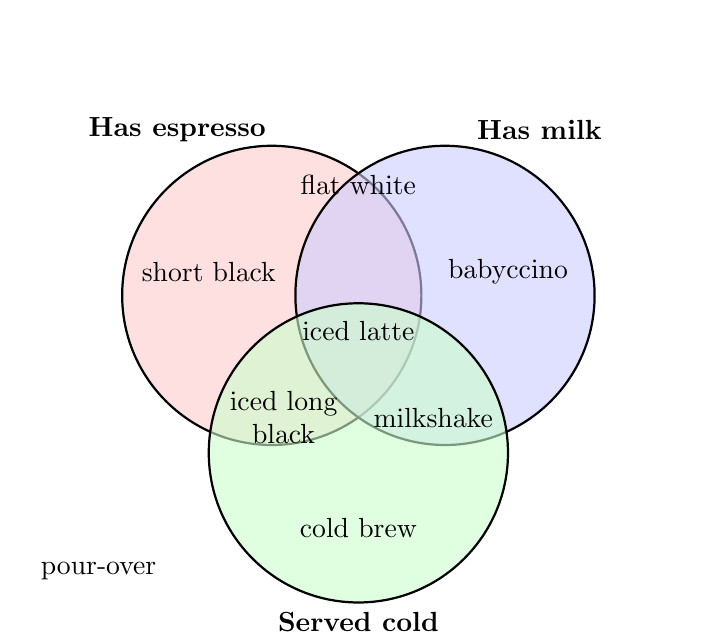
\begin{tikzpicture}
  % bounding box
  \useasboundingbox (-4.2,-3.2) rectangle (4.2,4.2);
  % Circles
  \draw[thick,fill=red!20,fill opacity=0.6] (-1.1,0.8) circle (1.9);
  \draw[thick,fill=blue!20,fill opacity=0.6] (1.1,0.8) circle (1.9);
  \draw[thick,fill=green!20,fill opacity=0.6] (0,-1.2) circle (1.9);
  % Labels
  \node[font=\bfseries] at (-2.3,2.9) {Has espresso};
  \node[font=\bfseries] at (2.3,2.9) {Has milk};
  \node[font=\bfseries] at (0,-3.35) {Served cold};
  % Drinks
  \node at (-1.9,1.1) {short black};
  \node at (0,2.2) {flat white};
  \node at (0,0.35) {iced latte};
  \node at (-0.95,-0.75) {\shortstack{iced long\\black}};
  \node at (0,-2.15) {cold brew};
  \node at (1.9,1.1) {babyccino};
  \node at (0.95,-0.75) {milkshake};
  \node at (-3.3,-2.7) {pour-over};
\end{tikzpicture}
\end{document}
